\documentclass[11pt]{nih}
%\usepackage[ascii]{inputenc}
\usepackage{amsmath}
\usepackage{amsfonts}
\usepackage{amssymb}
\usepackage{helvet}
\usepackage{algpseudocode}
\usepackage{algorithm}
\usepackage{url}
\usepackage{graphicx}
\date{}
%\renewcommand{\rmdefault}{phv}
\author{Ben Kandel}
\title{Sparse Methods for Dimensionality Reduction in Medical Imaging}
\begin{document}
\maketitle

\section*{Specific Aims}
In this proposal, we aim to advance sparse dimensionality reduction techniques in medical imaging to provide more accurate and robust correlations between imaging and cognitive and other clinical data.  This work falls under the following three aims. 
 
\subsection*{Specific Aim Ia:  Linear Sparse Medical Image Decomposition for Predicting Clinical Data} 
A variety of sparse matrix decomposition methods have been proposed that aim to reduce the dimensionality of a matrix while retaining non-zero entries on only a fraction of the basis vector entries.   Recently, supervised sparse decomposition methods tuned for images and other areas in which both spatial information and image labels are important have been developed.  We aim to extend this work to decompositions in which some clinical or other data that consists of a continuous variable is associated with each picture.  We also propose modifications of the smoothness constraints that are commonly used in matrix decompositions to both better preserve the reconstruction of the original data and also encourage anatomically interpretable basis vectors.  
\subsection*{Specific Aim Ib: Grouped Sparse Medical Image Decomposition}
In addition, we will examine the problem of incorporating prior anatomical knowledge into the decomposition, which is not typically a feature of sparse data decomposition.  We propose to use a group data decomposition algorithm.  This group algorithm will enforce sparsity only on labels (i.e., only a few pre-defined regions of the brain will be allowed to be included in the decomposition), but will not enforce sparsity \textit{within} a given region, so that within a region, all voxels of the region may vary freely.  This will encourage sparsity in an anatomically-informed way, so that anatomically meaningful regions as a whole will be allowed to stay in the model.  This can be seen as an ROI-based version of a sparse decomposition.
\subsection*{Specific Aim II: Non-Linear Sparse Dimensionality Reduction}
We propose to extend nonlinear dimensionality reduction techniques to the sparse setting.  Non-linear dimensionality reduction techniques are useful for analysis of data that does not lie on a linear subspace of the original, high-dimensional data.  Such nonlinear dimensionality reduction techniques have proven very useful in analysis of image data. In this work, we propose a sparse extension of one of the most popular non-linear dimensionality reduction techniques, Locally Linear Embedding (LLE).  We also demonstrate how the ideas presented here can be extended to the supervised decomposition problem. 
\subsection*{Specific Aim III: Application to Neurodegenerative Diseases}
Although the dimensionality reduction techniques outlined in the previous section are of general interest and can be applied to many types of image data, we are specifically interested in medical applications of the data.  Traditionally, medical image analysis is performed on a voxel-wise, mass univariate basis.  This technique, however, is not ideally suited for prediction of disease or clinical data because of the very high dimensionality of the analyzed data.  We propose to use the dimensionality reduction procedures outlined above to correlate specific areas  with decline in performance on cognitive tests in the setting of  Alzheimer's Disease. 

\section*{Background, Significance, and Innovation}
Medical imaging forms an increasingly indispensable role in medical diagnosis and disease characterization because it offers the ability to gain detailed information about the structure and function of patients' bodies.  At the same time, the richness and subtleties in medical images present significant methodological challenges for traditional statistical methodologies.  Because of the extremely high dimensionality and spatial information contained within medical images, traditional regression and classification techniques are not ideally suited for using medical images to make predictions as to a patient's disease state or clinical data.  Voxel-based morphometry (VBM) \cite{ashburner_voxel-based_2000}, one of the most widely used methods for analyzing neuroimaging data, looks for voxel-wise differences between groups of images.  Because the significance maps that are the output of VBM are still very high-dimensional, the output from VBM is not ideally suited to predictions of disease state or clinical data, and some other dimensionality reduction technique is still required \cite{batmanghelich_general_2009}.  In addition, because VBM operates in a mass-univariate manner, it can lose the ability to detect more subtle group differences that multivariate statistical methods are better suited to recover \cite{davatzikos_why_2004}.

Dimensionality reduction techniques are widely used to convert high-dimensional data into a low-dimensional space that in some way approximates the original high-dimensional data but that is more amenable to classification or other analytical tasks.  The methods are widely applied to a variety of data types, including facial images \cite{turk_eigenfaces_1991,belhumeur_eigenfaces_1997}, genetic data \cite{holter_fundamental_2000,yeung_principal_2001,alter_singular_2000,zou_sparse_2006,witten_penalized_2009}, and  medical images \cite{teipel_multivariate_2007}.  Classic dimensionality reduction techniques, such as Principal Components Analysis (PCA), however, have the drawback that the low-dimensional space is made up of contributions from every component in the high-dimensional space.  In the context of genetic analysis, this means that each principal component or eigenvector has non-zero entries that correspond to every gene in a gene array.  When using this low-dimensional space for looking for correlations between a given eigenvector and a clinical outcome, non-zero contributions from every gene in the gene array make it difficult to make biologically meaningful conclusions with regard to what any individual gene does.  In medical image analysis, a similar problem arises:  Non-zero entries in every  component in the principal components of a vector make it difficult to interpret which anatomical areas are most important for predicting a given clinical outcome.  

To alleviate this problem, one would try to find approximations to standard PCA decompositions that have a relatively small number of non-zero components.  Constraints on the number of non-zero components of a solution are referred to as \textit{sparsity} constraints, and the solutions of problems with sparsity constraints are referred to as sparse solutions.  Sparsity has been employed as a constraint in matrix decompositions in a wide variety of fields \cite{levy_reconstruction_1981,candes_robust_2006,zou_sparse_2006,sjostrand_sparse_2007,zhang_deformable_2011,witten_penalized_2009,zou_sparse_2006,jolliffe_simplified_2000,jolliffe_modified_2003,hoyer_non-negative_2004,batmanghelich_general_2009,batmanghelich_regularized_2011}.  Because of the close relationship between PCA and multivariate regression, techniques originally developed for regularizing linear regression, such as the Lasso and its variants \cite{tibshirani_regression_1996,tibshirani_sparsity_2005} can be profitably adapted to constraining PCA and other dimensionality reduction techniques, such as canonical correlation analysis (CCA) \cite{witten_extensions_2009}. 

Within this methodological context, we seek to tune existing strategies for dimensionality reduction techniques to the application of medical image analysis.  Although medical image matrix decompositions that take into account image labels have been proposed \cite{batmanghelich_general_2009}, none have been proposed that incorporate clinical data, such as a cognitive test, that consist of  continuous variables.  Incorporating  such continuous data into the decomposition will enable more robust detection of structural changes that are correlated with cognitive data.  Because cognitive tests are often designed to focus on one specific aspect of cognition, incorporating these data into the decomposition has the potential to shed light on which anatomical areas are correlated with which cognitive abilities in the context of neurodegenerative diseases.   At the same time, reducing the dimensionality of the input data will help ameliorate multiple comparisons issues and make linear regression models more powerful.  

A second aspect in which we will advance current methods in matrix decomposition involves the penalty terms used to ensure that the basis vectors obtained from the decomposition are anatomically meaningful. Most current matrix decomposition techniques in the field of medical imaging use a second-order smoothing term.  In many cases, however, first-order smoothing terms, such as those present in total variation denoising, have been found to outperform second-order smoothing terms when the data is known to contain large jumps \cite{rudin_nonlinear_1992}.  Because of the sparsity constraints on our basis vectors, we in fact do expect large jumps in the basis vectors, so first-order, or $\ell_1$, penalties on the vector derivatives are more appropriate.  We demonstrate how penalties of this sort have already been proposed for regularizing linear regression and show how they can be incorporated into a matrix decomposition framework.  

Existing sparse matrix decomposition methods for medical imaging also do not admit the possibility of incorporating prior knowledge, such as labels or region of interests (ROI's), into the decomposition.  We show how prior knowledge of anatomically meaningful areas can be incorporated into the decomposition to determine which anatomical regions show the most correlation with cognitive data. 

A second major class of dimensionality reduction techniques, in addition to the linear techniques discussed above, is nonlinear dimensionality reduction techniques.  Many forms of high-dimensional data, such as images, are not necessarily adequately explained by linear statistical techniques and are instead more aptly described as living on a non-linear manifold.  A wide variety of techniques have been proposed to deal with dimensionality reduction in this context, including kernelized versions of PCA \cite{scholkopf_kernel_1997} and manifold-based techniques \cite{tenenbaum_global_2000,roweis_nonlinear_2000,belkin_laplacian_2003,maaten_dimensionality_2008}.  Manifold-based techniques have been used effectively in analysis of neuroimaging data \cite{wolz_leap:_2010,wolz_nonlinear_2012}, but to date no sparse formulations have been proposed.  We propose a sparse extension to Locally Linear Embedding (LLE), one of the most widely used non-linear manifold-based dimensionality reduction techniques, and show how similar extensions may be made to other non-linear dimensionality reduction techniques.  Because manifold-based techniques do not involve mapping the input data to a higher-dimensional space, as in kernel methods, it is more straightforward to include spatially-informed priors on the basis vectors.  

Following the theoretical formulation of the dimensionality reduction techniques, we aim to implement the techniques and use them to analyze existing neuroimaging databases for connections between neuroanatomical variations and cognitive deficits.  Although a large body of research has focused on using anatomical or functional imaging for predicting the presence or absence of Alzheimer's Disease based on MRI scans, relatively few studies have used  sparse multivariate techniques similar to those proposed here to predict cognitive scores from neuroimaging scans.  Our methods have the potential to find areas of the brain that are maximally effective for predicting cognitive scores, and extensive testing, such as that proposed here, will both offer the opportunity to find novel neurobiological results and also demonstrate the power of the proposed methods to other researchers interested in using these methods.  

\subsection*{Notation}
To avoid confusion, we will describe the notation we use.  Matrices are denoted by bold capitalized letters ($\mathbf{X}$). If indexed, matrices are still  bolded, so that the $i$'th matrix is $\mathbf{X}_i$. Vectors are capitalized and italicized, but not bolded ($V$).  The $i$-th column vector of a matrix is denoted by an capitalized letter with a subscript  ($X_i$), and the entry corresponding to row $i$ and column $j$ is $x_{ij}$.    Scalars are lower-case ($x$), and sets in script ($\mathcal{N}$).  In keeping with standard usage, Greek letters used to denote vectors are not  capitalized, but the intent should be clear from the context.   Estimated values are given hats ($\hat{v}$).  The $\ell_p$ norms $\|x\|_p$ are defined as $\left( \sum_{i=1}^n \vert x_i \vert ^p \right) ^{1/p}$, with the $\ell_0$ pseudo-norm returning the number of non-zero entries in a vector.
 
\section*{Specific Aim I: Regression-Based and Grouped Sparse Linear Medical Image Decomposition}
\subsection*{Regression-Based Image Decomposition}
In order to fully appreciate how clinical data can be used to guide medical image decomposition, we will begin by briefly reviewing methods for sparse PCA decompositions.  Once we have shown how unsupervised sparse PCA decompositions are formulated, we will extend the decomposition to situations in which we have outcome data of a continuous variable. 

We represent a set of $n$ mean-centered medical images, each containing $p$ voxels, as an $n \times p$ matrix $\mathbf{X} \in \mathbb{R}^{n \times p}$.  We seek a decomposition of this matrix into a basis matrix $\mathbf{V} \in \mathbb{R}^{p \times r}$ and a loading matrix $\mathbf{W} \in \mathbb{R}^{r \times n}$  so that 
\begin{equation}
\mathbf{X}^{\mathrm{T}} \approx \mathbf{VW}.
\end{equation}
Two  common ways of formulating the PCA objective are finding the projection matrix $\mathbf{V}$ that maximizes the variance of the data matrix,
\begin{equation}
\hat{\mathbf{V}} =  \underset{\mathbf{V}}{\operatorname{arg\,max}} \, \| \mathbf{XV} \|_2^2,
\end{equation}
and finding the projection matrix that minimizes the reconstruction error, 
\begin{equation}
\mathbf{\hat{V}} = \underset{\mathbf{V}} {\operatorname{arg \,  min}} \, \| \mathbf{X} - \mathbf{VV}^{\mathrm{T}}  \mathbf{X}\|_2^2,
\label{eqn:reconstruction_error}
\end{equation}
subject to the orthogonality constraint $\mathbf{V}^{\mathrm{T}}\mathbf{V}=\mathbf{I}$, where $\mathbf{I}$ is the identity matrix \cite{hastie_elements_2009}.
The loading matrix is given by the projections of the data matrix onto the principal components
\begin{equation}
\mathbf{W} = \mathbf{XV},
\end{equation}
with matrix dimensions as before. 

Enforcing a sparsity constraint on this decomposition amounts to introducing a penalty on number of non-zero terms in the solution, which is known as the  $\ell_0$ pseudo-norm.  Because enforcing constraints on the $\ell_0$ pseudo-norm is in general an NP-hard problem \cite{natarajan_sparse_1995}, a standard convex relaxation is to introduce a penalty on the $\ell_1$ norm instead.  In many cases, this norm actually gives equivalent solutions \cite{donoho_for_2006}.   In the context of linear regression, the $\ell_1$ penalty is commonly known as the ``Lasso'' penalty \cite{tibshirani_regression_1996}, and Zou \cite{zou_sparse_2006} introduced this penalty into the PCA objective function (Equation \ref{eqn:reconstruction_error}) to obtain a sparse version of PCA. To do this, he used two matrices, $\mathbf{A}$ and $\mathbf{B}$, for use in the reconstruction, and then imposed orthogonality on $\mathbf{A}$ and sparsity on $\mathbf{B}$: 
\begin{equation}
(\hat{\mathbf{A}},\hat{\mathbf{B}}) = \underset{\mathbf{A},\, \mathbf{B}} {\operatorname{arg\,min}}  \| \mathbf{X} - \mathbf{A} \mathbf{B}^{\mathrm{T}} \mathbf{X}\|_2^2 + \lambda \| \mathbf{B}\|_1,
\end{equation}
subject to $\mathbf{A}^{\mathrm{T}} \mathbf{A} = I$.  The $\hat{\mathbf{B}}$ obtained from this equation will then satisfy $\hat{\mathbf{B}}_i \propto  \mathbf{V}_i$.  In addition to the sparsity constraint, some sort of clustering or smoothing penalty is required to avoid returning scattered non-zero components, as in \cite{batmanghelich_general_2009}.  This gives us an objective function of the form 
\begin{equation}
(\hat{\mathbf{A}},\hat{\mathbf{B}}) = \underset{\mathbf{A},\, \mathbf{B}} {\operatorname{arg\,min}}  \| \mathbf{X} - \mathbf{A} \mathbf{B}^{\mathrm{T}} \mathbf{X}\|_2^2 + \lambda_1 \| \mathbf{B}_j\|_1 + \lambda_2 p(\mathbf{B}),
\label{eqn:spca}
\end{equation}
where $p(\cdot)$ is some penalty that discourages spatially incoherent structures and and $\lambda_1$ and $\lambda_2$ are parameters that control the amount of sparsity and penalty for spatially incoherent structures, respectively.  

To encourage the basis vectors to contain non-zero entries that are grouped into anatomically coherent regions, a smoothing term is often applied to the decomposition.  Current methods in medical image decompositions (\cite{batmanghelich_general_2009,hebiri_smooth-lasso_2011}, following \cite{zdunek_blind_2008}) use a second-order smoothing term, such as $\sum_{j \in \mathcal{N}_i} \left(x_i - x_j\right)^2$, where $\mathcal{N}_i$ is the neighborhood of voxels adjacent to $x_i$.  Second-order smoothing terms, however, penalize large discontinuities much more than small discontinuities.  Because we are interested in enforcing sparseness in our solution, we will necessarily be interested in possibly large non-zero entries next to wide areas of zero entries.  An $\ell_1$ norm on the gradient, such as that adopted in total variation-based denoising \cite{rudin_nonlinear_1992}, is more appropriate for our application, because it penalizes large jumps less than $\ell_2$ norms.  In the context of linear regression, this penalty is known as the ``fused Lasso'' \cite{tibshirani_sparsity_2005}, and has the form $ \lambda_2 \sum_{j \in \mathcal{N}_i} |x_i - x_j|$, when $\mathcal{N}_i$ is the neighborhood of $x_i$.  Adding this penalty explicitly to Equation \ref{eqn:spca} (and adjusting the neighborhood for two-dimensional matrices) gives us 
\begin{equation}
(\hat{\mathbf{A}},\hat{\mathbf{B}}) = \underset{\mathbf{A},\, \mathbf{B}} {\operatorname{arg\,min}}  \| \mathbf{X} - \mathbf{A} \mathbf{B}^{\mathrm{T}} \mathbf{X}\|_2^2 + \lambda_1 \| \mathbf{B}\|_1  + \lambda_2 \sum_{j=1}^p \sum_{k=1}^r \sum_{\left\lbrace m,n \mid b_{mn} \in \mathcal{N}_{jk} \right\rbrace} \vert b_{jk} -b_{mn} \vert .
\end{equation} 

A second extension I propose is to incorporate regression of the projections onto the available clinical data in the objective function.  The clinical data can take the form of cognitive scores, disease state (in logistic regression), or other outcomes one is trying to predict.  This can be considered a generalization of the classification loss term considered by \cite{batmanghelich_general_2009}.  Denoting the regression coefficients $\beta$, so that the standard multivariate regression equation is $Y = \mathbf{X} \beta$, we can then finally write 
\begin{equation}
(\hat{\mathbf{A}},\hat{\mathbf{B}}) = \underset{\mathbf{A},\, \mathbf{B}} {\operatorname{arg\,min}}  \| \mathbf{X} - \mathbf{A} \mathbf{B}^{\mathrm{T}} \mathbf{X}\|_2^2 + \lambda_1 \| \mathbf{B}\|_1  + \lambda_2 \sum_{j=1}^p \sum_{k=1}^r \sum_{\left\lbrace m,n \mid b_{mn} \in \mathcal{N}_{jk} \right\rbrace} \vert b_{jk} -b_{mn} \vert + \lambda_3 \| Y - \mathbf{XB} \beta \|_2^2
\end{equation}
Incorporating a loss term based on the prediction of the clinical data will encourage the decomposition to be correlated with the clinical outcomes, and changes the unsupervised decomposition to a supervised decomposition reminiscent of partial least squares regression.  

Another aspect in which we aim to modify current sparse image decompositions is in how prior information is incorporated into the decompositions. Although the penalties proposed do encourage the decomposition to correspond to regions that \textit{can} be anatomically meaningful (coherent, smooth, etc.), the projections may still spread over distinct anatomical regions.  I propose to introduce a modified version of the decomposition that will incorporate prior anatomical knowledge in the form of a labeled atlas.  At the same time, we are still interested in decompositions that do not spread over the entire brain.  We are interested in having a limited number of predefined regions in the brain, but within those regions do not have further sparsity constraints.   In other words, we are interested in region-wise sparsity, but not voxel-wise sparsity.  This problem is a model selection problem, and many techniques have been developed for solving similar problems.  One possible greedy example, based on partial least squares regression and incorporating Tikhonov (or ridge) regularization, is proposed in Algorithm \ref{alg:selection}.  

\begin{algorithm}
\begin{algorithmic}
\State \textbf{Input}: $\mathbf{V},\mathbf{X},Y$. \Comment{Input labeled regions, image matrix, clinical outcome.}
\State $i \leftarrow 1$.  \Comment{ Initialize iterator.}
\While{adding additional regions improves model}
\State $\left(Q_i, \hat{\mathbf{B}_i}, \hat{\beta_i} \right) \leftarrow \underset{V_i, \mathbf{B}_i, \beta_i}{\operatorname{arg\,min}} \| V_i V_i^{\mathrm{T}} \mathbf{X} - \mathbf{B}_i \mathbf{B}_i^{\mathrm{T}} V_i V_i^{\mathrm{T}} \mathbf{X}  \|_2^2 + \|Y - V_i V_i^{\mathrm{T}} \mathbf{X} \beta \|_2^2 + \lambda \|\beta_i\|_2^2 $ \Comment{Find region whose partial least squares regression solution gives greatest correlation with output and add to model.} 
\State $Y \leftarrow Y - V_i V_i^{\mathrm{T}} \mathbf{X} \beta$. \Comment{Retain only clinical data unexplained by current model.}
\State $i \leftarrow i + 1$. 
\EndWhile
\State \textbf{Output}: $\mathbf{Q}, \beta$ \Comment{Return regions selected for model with coefficients for predicting clinical scores.}
\end{algorithmic}
\caption{Algorithm for selecting most significant regions for predicting cognitive scores.}
\label{alg:selection}
\end{algorithm}



Denoting each brain region as $\mathbf{V}_j$, with all the brain region vectors incorporated into a matrix $\mathbf{V}$ and the projection of the images onto all the brain regions as $\mathbf{XV}^{\mathrm{T}}$, we then have an objective of the form 
\begin{equation}
\| y - \mathbf{XV}^{\mathrm{T}}  \gamma \| + \lambda \| \gamma \|^2 + p(k),
\end{equation}
when $k$ is the number of regions incorporated into the model and $p(k)$ is a penalty on the number of regions incorporated into the model.   The $\ell^2$ regularization on $\gamma$ is the standard ridge (or Tikhonov) regularization necessary to avoid degenerate solutions. This objective turns in to a modified model selection problem, and a wide variety of methods are available to find (local) minima.  

Perhaps the simplest method for solving this problem involves a  greedy selection algorithm.  A greedy algorithm would first choose the region $V_i$, corresponding to one column in $\mathbf{V}$, with the highest correlation with the outcome variable:
\begin{equation}
\left(\hat{V}_i, \gamma_i \right) = \underset{V_i, \gamma_i}{\operatorname{arg \, min}} \| y - \mathbf{X} {\operatorname{diag}} (V_i) \gamma_i \|^2, 
\end{equation}
 where ${\operatorname{diag}}(x)  : x \in \mathbb{R}^m \rightarrow X \in \mathbb{R}^{m \times m}$ takes a vector $x \in \mathbb{R}^m$ and creates an $m \times m$ matrix with diagonal entries equal to entries in $x$.   Next, it would find the region with the highest correlation with the residual (i.e., the response not accounted for by the region already included in the model): 
\begin{equation}
\left(\hat{V}_{i+1}, \gamma_{i+1} \right) = \underset{V_{i+1}, \gamma_{i+1}}{\operatorname{arg \, min}} \| y - \mathbf{X} {\operatorname{diag}} (V_i) \gamma_i  - \mathbf{X} {\operatorname{diag}} (V_{i+1}) \gamma_{i+1} \|^2
\end{equation} 
We would then test if incorporating the extra region significantly improves the model, as determined by whether or not the BIC score  \cite{schwarz_estimating_1978} decreases with the added region.  



More sophisticated group model selection algorithms have also been proposed.  Grouped versions of the Lasso and Least Angle Regression (LARS) \cite{efron_least_2004} have been proposed to deal with this type of problem \cite{yuan_model_2006}.  The group version of LARS performs the following steps:  First, it picks the group of variables that is most correlated with the outcome variable.  It then moves the solution in this direction until the projection of the residual of the outcome (i.e., the outcome not explained by the current model) onto another group has as small an angle with the outcome as the original direction has with the outcome.  Subsequent groups are added in a similar way until some stopping criterion is met.  The stopping criterion can be some threshold on prediction error or some other metric, such as the BIC, that takes into account model size.

Now that we have laid out some of the specific mathematical forms that we will be optimizing, we will reiterate the significance of the proposed methods for medical image analysis.  The fundamental issue that confronts analysis of medical image data is the extremely high dimensionality of the input data.  Because of this high dimensionality, some dimensionality reduction method is necessary to make meaningful correlations with clinical or other data.  First, we proposed an unsupervised dimensionality reduction technique that takes into account anatomically meaningful constraints to ensure that the output vectors can be meaningfully interpreted.  Next, we extended this model to encourage the decomposition to be correlated with available clinical data.  Finally, we outlined a method for incorporating prior anatomical knowledge into the decomposition.  This method has the practical effect of enabling a researcher to determine which anatomical regions, out of a set of predefined regions, are most important for predicting some clinical outcome.  In all these methods, sparsity is incorporated as a constraint to make sure that the model corresponds to only certain portions of the anatomy, and does not spread over the entire image.  Until now, though, we have assumed that the clinical data can be modeled as a multivariate linear function of the input images.  In the next section, we will see how it may be possible to relax that assumption and still obtain sparse decompositions. 

\section*{Specific Aim II: Non-Linear Sparse Dimensionality Reduction}
\begin{figure}
\centering
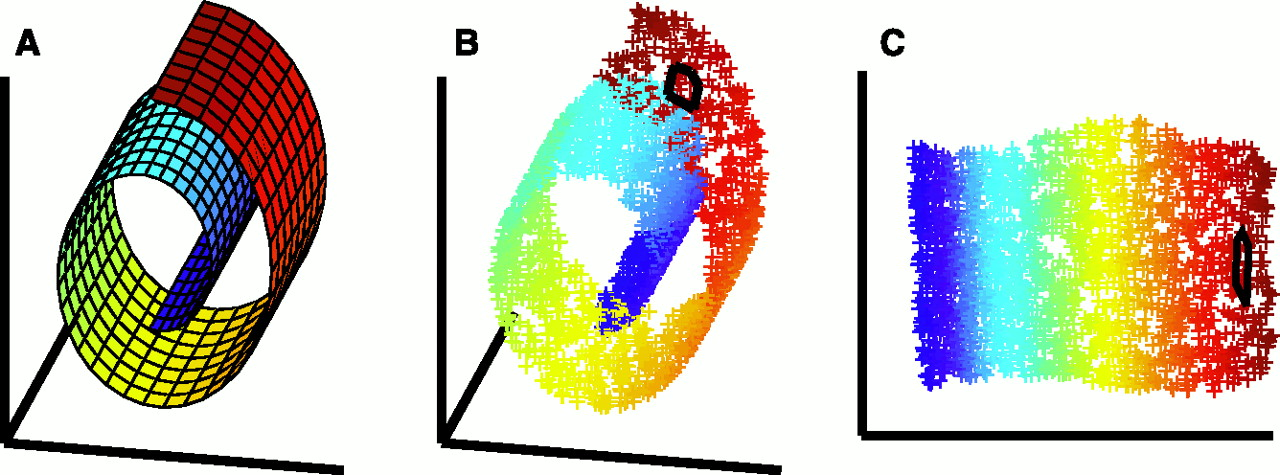
\includegraphics[width=10cm]{swiss_roll.jpg}
\caption{Demonstration of ``Swiss roll'' data that demonstrates the utility of non-linear dimensionality reduction techniques.  The data cannot be satisfactorily explained by a linear projection, but the non-linear manifold dimensionality reduction technique Locally Linear Embedding (LLE) successfully ``unwraps'' the curve and presents a reasonable two-dimensional decomposition of the data.  Figure taken from \cite{roweis_nonlinear_2000}.}
\label{fig:swiss}
\end{figure}
Although the multivariate linear dimensionality reduction techniques proposed above will enable recovery of linear correlations between imaging data and clinical or other data, they will not be able to perform non-linear dimensionality reduction (Figure \ref{fig:swiss}).  As an example technique, we will propose a sparse extension to Locally Linear Embedding (LLE), one of the most widely used non-linear dimensionality reduction techniques.  Building on recent extensions of LLE to the supervised learning context, we will propose both an unsupervised and a supervised dimensionality reduction technique.   The practical performance of the various manifold and other non-linear dimensionality reduction techniques is heavily application-dependent, but the widespread use and straightforward implementation of LLE makes it a reasonable place to start for proposing a sparse extension.  

LLE works by computing the following three steps: 
\begin{enumerate}
\item For each data point $X_i$, find a neighborhood $\mathcal{N}_i$ of other data points that are most similar to it.  Assignments can be made by $k$-nearest neighbors or by incorporating all neighbors such that the distance between $X_i$ and its neighbors is less than some $\epsilon$. 
\item Determine optimal reconstruction weights to reconstruct each data point $X_i$ from its neighbors by minimizing the reconstruction error
\begin{equation} 
\varepsilon \left(W\right) = \underset{W} {\operatorname{arg \, min}} \sum_i \| X_i - \sum_{j \in \mathcal{N}_i}W_{ij}X_j \|^2.
\label{eqn:lle_reconstruction}
 \end{equation}
\item With weights fixed, find the low-dimensional embedding that most closely approximates the high-dimensional weight structure: $\Phi \left(Y \right) = \sum_i \|Y_i - \sum_{j \in \mathcal{N}_i} W_{ij}Y_j \|^2$. 
\end{enumerate}
To see how we can extend this method to incorporate sparsity, we will briefly review linear sparse PCA.  The reconstruction errorformulation of PCA seeks to find a vector which will minimize the reconstruction error of the matrix $\mathbf{X}$: 
\begin{equation}
\hat{v} = \underset{v}{\operatorname{arg\, min}} \| \mathbf{X} - v v^{\mathrm{T}} \mathbf{X}\|
\end{equation}
This equation is similar to the reconstruction weight equation (Equation \ref{eqn:lle_reconstruction}), except that Equation \ref{eqn:lle_reconstruction} only utilizes the data points in the neighborhood of the target image.  From a sparse version of LLE, we would hope to recover both the reconstruction weights (so that we can compute a low-dimensional embedding) and the vector that specifies a section of the original matrix that is most critical for the LLE reconstruction.  In the simplest case, this would correspond to a Boolean vector $v$ whose entries belong to the set $\lbrace 0,1 \rbrace$, which would give us a reconstruction error of the form 
\begin{equation}
\varepsilon_{sparse} \left( W, v \right) = \underset{W, v}{\operatorname{arg\, min}} \sum_i \|X_i - \sum_{j \in \mathcal{N}_i} W_{ij} \left(v \odot X_j \right) \|^2,
\end{equation}
 where $\odot$ stands for element-wise multiplication.  However, optimizing over Boolean vectors is generally very difficult, so we will relax this constraint and reformulate the problem in terms of a change of basis that is more similar to the sparse PCA formulation discussed above. 
 
Modifying Equation \ref{eqn:lle_reconstruction} in this way gives us 
\begin{equation}
\varepsilon_{sparse} \left(W, v\right) = \underset{W, v}{\operatorname{arg\, min}} \sum_i \| X_i - \sum_{j \in \mathcal{N}_i}W_{ij} v v^{\mathrm{T}} X_j \|^2.
\label{eqn:sparse_lle}
\end{equation}
When $v$ is the identity matrix, Equation \ref{eqn:sparse_lle} is clearly equivalent to Equation \ref{eqn:lle_reconstruction}, but we are interested in incorporating sparsity in the form of an $\ell^1$ penalty on the solution: 
\begin{equation}
\varepsilon_{sparse} \left(W, v\right) = \underset{W,v}{\operatorname{arg\, min}}\sum_i \| X_i - \sum_{j \in \mathcal{N}_i}W_{ij} v v^{\mathrm{T}} X_j \|^2 + \|v\|_1,
\end{equation}
where as before, $v$ is orthogonal.  Note that the $v$ matrix is not indexed.  This objective will return a PC-like sparse matrix that is best suited to reconstructing each individual data point from a weighted combination of its neighbors.  The sparse matrix will then indicate which parts of the image, or in our case, which anatomical component, is most important for reconstruction of the original image.  The connections between this decomposition and the linear sparse decomposition methods described above are clear; the difference is that in this case, we only consider the reconstruction of each data point based on the data points (or images) that are most similar to it.  

To extend this decomposition to the supervised domain, we must take into account some clinical data by incorporating the available labels into the decomposition.  A variety of supervised versions of manifold-based non-linear dimensionality reduction techniques have been proposed for greater discrimination power between members of different groups \cite{kaynak_supervised_????,yang_extended_2002,geng_supervised_2005,raducanu_supervised_2012} .  The basic idea is to define the distance (in step 1) between data points from within the same class differently from distances between data points in different classes.  By incorporating class information into the decomposition, a greater degree of discrimination is possible between data points from different classes.  In its simplest form, it consists of simply adding a constant to distances between data points between different classes \cite{kaynak_supervised_????}, but more sophisticated versions are possible that give greater control over the distance between images from different classes. Incorporating class labels may improve the ability of the low-dimensional embedding to preserve distinctions between images of different classes, which will improve the ability to classify unseen images.  

Once a low-dimensional embedding is computed, it is possible to use the low-dimensional embedding to predict clinical data in either a  regression-type or classification-type framework.  We leave the possibility of incorporating continuous data into the decomposition to future research.  

\section*{Specific Aim III: Validation and Clinical Application}
Although the theoretical formulations above are necessary to be able to perform the decompositions, the ultimate utility of the proposed decomposition methods depends on their performance on actual data sets.  We will begin the practical evaluation of the methods proposed by implementing them in Matlab and evaluating their performance on synthetic datasets.  In the first stage, we will generate synthetic datasets by forming images with simple geometric shapes, such as circles.  We will then introduce a perturbation, such as an area of increased brightness, in some of the images.  Synthetic ``clinical'' data may consist of a value that scales linearly with the intensity of perturbation in the test images.  The sparse PCA algorithm should be able to retrieve the area of perturbation, and this will serve as the first stage of validation that the algorithm has been correctly implemented.  After this initial test of the linear dimensionality reduction techniques, we can extend the validation by changing the shape of the perturbation and adding scattered points of perturbation to test the effect of the various weighting parameters that encourage the PCA algorithm to find smooth eigenvectors.  

Following validation of the linear dimensionality reduction algorithms, we will implement the non-linear sparse dimensionality reduction algorithm.  As a set of test images for algorithm, we propose to use existing image datasets.  The image sets generated for testing Isomap \cite{tenenbaum_global_2000} are freely available \url{http://isomap.stanford.edu/datasets.html} and will be a good place to perform preliminary testing.  

After the initial validation and debugging of the implementations are complete, we aim to move towards analysis of neuroimaging data.  To work with neuroimaging data, it is usually necessary to use a lower-level language than Matlab to avoid limits on memory usage and to improve speed.  We aim to implement the algorithms in the \verb=sccan= program, which is part of the ANTs software developed by PICSL.  Matrix manipulations are performed using the VNL matrix operation library, which is integrated into ITK for processing medical images.  

For test data, we propose to analyze two independent sets of Alzheimer's Disease patients.  First, we will use the publicly available Alzheimer's Disease Neuroimaging Initiative, which has a large dataset of both imaging and clinical data.  We will also perform the analysis on a large dataset of AD and control patients available from the University of Pennsylvania Memory Center, which has a more ethnically and demographically varied subject group than the ADNI dataset.  Performing the analysis on two independently collected sets of data will augment our confidence that any neurobiological results we find constitute meaningful and robust results. Using the modified linear regression techniques proposed above will enable probing the connection between individual brain structures and clinical scores.  We will examine the connection between cortical thickness and scores on the Boston Naming Test (BNT), a test of language and recall function; the Trail-Making test, a test of cognitive processing speed (part A) and executive function (part B) ability \cite{bowie_administration_2006}; and the Mini-Mental State Exam (MMSE).  Both the dataset from the Penn Memory Center and the ADNI data have these tests available. 

\bibliographystyle{plain}
\bibliography{kandel_lib}
\end{document}